%---------------------------------------------------------------------------%
%-                                                                         -%
%-                           LaTeX Template                                -%
%-                                                                         -%
%---------------------------------------------------------------------------%
%- Copyright (C) Huangrui Mo <huangrui.mo@gmail.com>
%- This is free software: you can redistribute it and/or modify it
%- under the terms of the GNU General Public License as published by
%- the Free Software Foundation, either version 3 of the License, or
%- (at your option) any later version.
%---------------------------------------------------------------------------%
%->> Document class declaration
%---------------------------------------------------------------------------%
\documentclass[printcopy,fontset=windows]{Style/neuthesis}%
%- Multiple optional arguments:
%- [<singlesided|doublesided|printcopy>]% set one or two sided eprint or print
%- [draftversion]% show draft version information
%- [fontset=<fandol|windows|mac|adobe>]% specify font set to replace automatic detection
%- [scheme=plain]% thesis writing of international students
%- [standard options for ctex book class: draft|paper size|font size|...]%
%---------------------------------------------------------------------------%
%->> Document settings
%---------------------------------------------------------------------------%
\usepackage[bibtex,myhdr,table,list,geometry,math]{Style/artratex}
% document settings
%- usage: \usepackage[option1,option2,...,optionN]{artratex}
%- Multiple optional arguments:
%- [bibtex|biber]% set bibliography processor and package
%- [geometry]% reconfigure page layout via geometry package
%- [lscape]% provide landscape layout environment
%- [myhdr]% enable header and footer via fancyhdr package
%- [color]% provide color support via xcolor package
%- [background]% enable page background
%- [tikz]% provide complex diagrams via tikz package
%- [table]% provide complex tables via ctable package
%- [list]% provide enhanced list environments for algorithm and coding
%- [math]% enable some extra math packages
\usepackage{Style/artracom}% user defined commands
%---------------------------------------------------------------------------%
%->> Document inclusion
%---------------------------------------------------------------------------%
%\includeonly{Tex/Chap_1,...,Tex/Chap_N}% selected files compilation
%---------------------------------------------------------------------------%
%->> Document content
%---------------------------------------------------------------------------%
\def\alltex{}
\begin{document}
% \layout
%-
%-> Frontmatter: title page, abstract, content list, symbol list, preface
%-
\frontmatter% initialize the environment
% !TEX ROOT = ../Thesis.tex 
%---------------------------------------------------------------------------%
%->> 封面信息及生成
%---------------------------------------------------------------------------%
%-
%-> 中文封面信息
%-
\category{}%分类号
\confidential{}% 密级:只有涉密论文才填写
\UDC{}
\schoollogo% 校徽
% \schooltitle{width=1cm}{neu_title}
\title{东北大学博士学位论文排版打印格式}% 论文中文题目
\author{xxx}% 论文作者
\advisor{xx~~教授}% 指导教师:姓名 专业技术职务 工作单位
\advisorsec{东北大学计算机科学与工程学院}% 指导老师附加信息 或 第二指导老师信息
\degree{博士}% 学位:学士、硕士、博士
\degreetype{工学}% 学位类别:理学、工学、工程、医学等
\major{计算机应用技术}% 二级学科专业名称
\institute{计算机科学与工程学院}% 院系名称

\research{网络空间安全}% 研究方向
\authorno{1910411}% 学号
\chinesedate{2019~年~4~月}%  封面页脚日期
\submissiondate{2018~年~12~月}% 论文提交日期
\oraldefencedate{2019~年~3~月}% 论文答辩日期
\degreedate{2019~年~4~月}% 学位授予日期
\chairman{xxx}% 答辩委员会主席
%-
%-> 英文封面信息
%-
\englishtitle{Thesis Template of Northeastern University}% 论文英文题目
\englishauthor{Wang xx-xx}% 论文作者
\englishadvisor{Professor Zhao xxx}% 指导教师
\englishdegree{Doctor}% 学位:Bachelor, Master, Doctor。封面格式将根据英文学位名称自动切换,请确保拼写准确无误
\englishdegreetype{Natural Science}% 学位类别:Philosophy, Natural Science, Engineering, Economics, Agriculture 等
\englishthesistype{thesis}% 论文类型: thesis, dissertation
\englishuniversity{Northeastern University}
\englishmajor{Computer Application Thechnology}% 二级学科专业名称
\englishinstitute{School of Computer Science and Engineering}% 院系名称
\englishdate{April 2019}% 毕业日期:春季 April 夏季为June、秋季为September 冬季为December
%-
%-> 生成封面
%-
\makereviewcover % 生成盲审中文封面
\makeprintcover %生成打印的中文封面
\makechinesetitle % 生成中文内容页
\makeenglishtitle% 生成英文页
%-
%-> 作者声明
%-
\makedeclaration% 生成声明页
% title page, abstract, dedication
% !TEX ROOT = ../Thesis.tex 
%-
%-> 中文摘要
%-
\chapter{摘\quad 要}\chaptermark{摘\quad 要}% 摘要标题
% \setcounter{page}{1}% 开始页码
% \pagenumbering{Roman}% 页码符号
% 22p / 12p = 1.83
\linespread{1.5}
\zihao{-4}
% \setlength{\baselineskip}{20pt}

本文是东北大学博士学位论文Latex模板使用说明文档

\keywords{东北大学; Latex模板; 说明文档;}% 中文关键词
%-
%-> 英文摘要
%-
\chapter{Abstract}\chaptermark{Abstract}% 摘要标题

This is a help documentation of Latex template for the Ph.D. thesis in Northeastern University.

\englishkeywords{Northeastern University; Latex Template; Help documentation;}
 % abstract (chinese and english)

{% content list region
% \linespread{1}
% \intotoc{\contentsname}% add link to contents table and bookmark
% \chapter*{\contentsname}
\linespread{1.5}% local line space
\tableofcontents% contents catalog

\intotoc{\listfigurename}% add link to contents table and bookmark
\listoffigures% figures catalog

\intotoc{\listtablename}% add link to contents table and bookmark
\listoftables% tables catalog
}
% \input{Tex/Prematter}% list of symbols, preface content
%-
%-> Mainmatter
%-
\mainmatter% initialize the environment
\linespread{1.4}
\zihao{-4}
%---------------------------------------------------------------------------%
%->> Main content
%---------------------------------------------------------------------------%
\chapter{绪论}\label{chap:introduction}

\section{背景}

考虑到许多同学可能缺乏\LaTeX{}使用经验,neuthesis将\LaTeX{}的复杂性高度封装,开放出简单的接口,以便轻易使用。同时,对用\LaTeX{}撰写论文的一些主要难题,如制图、制表、文献索引等,进行了详细说明,并提供了相应的代码样本,理解了上述问题后,对于初学者而言,使用此模板撰写学位论文将不存在实质性的困难。所以,如果你是初学者,请不要直接放弃,因为同样为初学者的我,十分明白让\LaTeX{}简单易用的重要性,而这正是neuthesis所追求和体现的。

该模板基于中国科学院大学学位论文模板causthesis模板发展而来。neuthesis模板满足最新的东北大学博士学位论文排版要求和封面打印设定。兼顾操作系统:Windows,Linux,MacOS 和\LaTeX{}编译引擎:pdflatex,xelatex,lualatex。支持中文书签、中文渲染、中文粗体显示、拷贝PDF中的文本到其他文本编辑器等特性。此外,对模板的文档结构进行了精心设计,撰写了编译脚本提高模板的易用性和使用效率。

neuthesis的目标在于简化学位论文的撰写,利用\LaTeX{}格式与内容分离的特征,模板将格式设计好后,作者可只需关注论文内容。 同时,neuthesis有着整洁一致的代码结构和扼要的注解,对文档的仔细阅读可为初学者提供一个学习\LaTeX{}的窗口。

\section{系统要求}\label{sec:system}

\href{https://github.com/mervin0502/neuthesis}{\texttt{neuthesis}} 宏包可以在目前主流的 \href{https://en.wikibooks.org/wiki/LaTeX/Introduction}{\LaTeX{}} 编译系统中使用,例如C\TeX{}套装 (请勿混淆C\TeX{}套装与ctex宏包。C\TeX{}套装是集成了许多\LaTeX{}组件的\LaTeX{}编译系统,因已停止维护,\textbf{不再建议使用}。 \href{https://ctan.org/pkg/ctex?lang=en}{ctex} 宏包如同neuthesis,是\LaTeX{}命令集,其维护状态活跃,并被主流的\LaTeX{}编译系统默认集成,是几乎所有\LaTeX{}中文文档的核心架构。)、MiK\TeX{}(维护较不稳定,\textbf{不太推荐使用})、\TeX{}Live。推荐的 \href{https://en.wikibooks.org/wiki/LaTeX/Installation}{\LaTeX{}编译系统} 和 \href{https://en.wikibooks.org/wiki/LaTeX/Installation}{\LaTeX{}文本编辑器} 为

\LaTeX{}编译系统 (如\TeX{}Live) 用于提供编译环境,\LaTeX{}文本编辑器 (如Texmaker) 用于编辑\TeX{}源文件。请从各软件的官网下载安装程序,勿使用其它程序源。\textbf{\LaTeX{}编译系统和\LaTeX{}编辑器分别安装成功后,用户即完成了\LaTeX{}的系统配置},无需其他手动干预和配置。若用户的系统原带有旧版的\LaTeX{}编译系统并想安装新版,请\textbf{先卸载干净旧版再安装新版}。

\section{问题反馈}

关于\LaTeX{}的知识性问题,请查阅 
\href{https://github.com/mohuangrui/ucasthesis/wiki}{\LaTeX{}知识小站} 和 
\href{https://en.wikibooks.org/wiki/LaTeX}{\LaTeX{} Wikibook}。

关于模板编译和样式设计的问题,请\textbf{先仔细阅读此说明文档,特别是“常见问题”(章节~\ref{sec:qa})}。若问题仍无法得到解决,请\textbf{先将问题理解清楚并描述清楚,再将问题反馈}至 \href{https://github.com/mervin0502/neuthesis/issues}{Github/neuthesis/issues}。

欢迎大家有效地反馈模板不足之处,一起不断改进模板。希望大家向同事积极推广\LaTeX{},一起更高效地做科研。

\section{模板下载}

\begin{center}
    \href{https://github.com/mervin0502/neuthesis}{Github/neuthesis}: \url{https://github.com/mervin0502/neuthesis}
\end{center}


\chapter{LaTeX使用说明}\label{chap:guide}

为方便使用及更好地展示LaTeX排版的优秀特性,neuthesis的框架和文件体系进行了细致地处理,尽可能地对各个功能和板块进行了模块化和封装,对于初学者来说,众多的文件目录也许一开始让人觉得有些无所适从,但阅读完下面的使用说明后,会发现原来使用思路是简单而清晰的,而且,当对LaTeX有一定的认识和了解后,会发现其相对Word类排版系统极具吸引力的优秀特性。所以,如果是初学者,请不要退缩,请稍加尝试和坚持,以领略到LaTeX的非凡魅力,并可以通过阅读相关资料如LaTeX Wikibook\cite{wikibook2014latex}来完善自己的使用知识。

\section{先试试效果}

\begin{enumerate}
    \item 安装软件:根据所用操作系统和章节~`\ref{sec:system}`中的信息安装LaTeX编译环境。
    \item 获取模板:下载 \href{https://github.com/mervin0502/neuthesis}{neuthesis} 模板并解压。neuthesis模板不仅提供了相应的类文件,同时也提供了包括参考文献等在内的完成学位论文的一切要素,所以,下载时,推荐下载整个neuthesis文件夹,而不是单独的文档类。
    \item 编译模板:
        \begin{enumerate}
            \item Windows:双击运行artratex.bat脚本。
            \item Linux或MacOS: {\scriptsize \verb|terminal| -> \verb|chmod +x ./artratex.sh| -> \verb|./artratex.sh xa|}
            \item 任意系统:都可使用LaTeX编辑器打开Thesis.tex文件并选择xelatex编译引擎进行编译。
        \end{enumerate}
    \item 错误处理:若编译中遇到了问题,请先查看“常见问题”(章节~\ref{sec:qa})。
\end{enumerate}

编译完成即可获得本PDF说明文档。而这也完成了学习使用neuthesis撰写论文的一半进程。什么?这就学成一半了,这么简单???,是的,就这么简单!

\section{文档目录简介}

\subsection{Thesis.tex}

Thesis.tex为主文档,其设计和规划了论文的整体框架,通过对其的阅读可以了解整个论文框架的搭建。

\subsection{编译脚本}

\begin{itemize}
    \item Windows:双击Dos脚本artratex.bat可得全编译后的PDF文档,其存在是为了帮助不了解LaTeX编译过程的初学者跨过编译这第一道坎,请勿通过邮件传播和接收此脚本,以防范Dos脚本的潜在风险。
    \item Linux或MacOS:在terminal中运行
        \begin{itemize}
            \item \verb|./artratex.sh xa|:获得全编译后的PDF文档
            \item \verb|./artratex.sh x|:快速编译模式
        \end{itemize}
    \item 全编译指运行 \verb|xelatex+bibtex+xelatex+xelatex| 以正确生成所有的引用链接,如目录,参考文献及引用等。在写作过程中若无添加新的引用,则可用快速编译,即只运行一遍LaTeX编译引擎以减少编译时间。
\end{itemize}

\subsection{Tmp文件夹}

运行编译脚本后,编译所生成的文档皆存于Tmp文件夹内,包括编译得到的PDF文档,其存在是为了保持工作空间的整洁,因为好的心情是很重要的。

\subsection{Style文件夹}

包含neuthesis文档类的定义文件和配置文件,通过对它们的修改可以实现特定的模版设定。若需更新模板,一般只需用新的样式文件替换旧的即可。

\begin{enumerate}
    \item neuthesis.cls:文档类定义文件,论文的最核心的格式即通过它来定义的。
    \item neuthesis.cfg:文档类配置文件,设定如目录显示为“目~录”而非“目录”。
    \item artratex.sty: 常用宏包及文档设定,如参考文献样式、文献引用样式、页眉页脚设定等。这些功能具有开关选项,常只需在Thesis.tex中的如下命令中进行启用即可,一般无需修改artratex.sty本身。
        
        \path{\usepackage[options]{artratex}} 
    \item artracom.sty:自定义命令以及添加宏包的推荐放置位置。
\end{enumerate}

\subsection{Tex文件夹}

文件夹内为论文的所有实体内容,正常情况下,这也是\textbf{使用neuthesis撰写学文论文时,主要关注和修改的一个位置,注:所有文件都必须采用UTF-8编码,否则编译后将出现乱码文本},详细分类介绍如下:

\begin{itemize}
    \item Frontpage.tex:为论文中英文封面及中英文摘要。\textbf{论文封面会根据英文学位名称如Bachelor,Master,或是Doctor自动切换为相应的格式}。
    \item Mainmatter.tex:索引需要出现的Chapter。开始写论文时,可以只索引当前章节,以快速编译查看,当论文完成后,再对所有章节进行索引即可。
    \item Chap{\_}xxx.tex:为论文主体的各个章节,可根据需要添加和撰写。
    \item Appendix.tex:为附录内容
    \item Backmatter.tex:为发表文章信息和致谢部分等。
\end{itemize}

\subsection{Img文件夹}

用于放置论文中所需要的图类文件,支持格式有:.jpg, .png, .pdf。其中,\verb|neu_logo.pdf|为东北大学校徽。不建议为各章节图片建子目录,即使图片众多,若命名规则合理,图片查询亦是十分方便。

\subsection{Biblio文件夹}

\begin{enumerate}
    \item ref.bib:参考文献信息库。
    \item gbt7714-xxx.bst:符合国标的文献样式定义文件。由 \href{https://github.com/zepinglee/gbt7714-bibtex-style}{zepinglee}  开发,并满足最新国标要求。与文献样式有关的问题,请查阅开发者所提供的文档,并建议适当追踪其更新。
\end{enumerate}

\section{常见使用问题}\label{sec:qa}

\begin{enumerate}
    \item 模板每次发布前,都已在Windows,Linux,MacOS系统上测试通过。下载模板后,若编译出现错误,则请见 \href{https://github.com/mervin0502/neuthesis/wiki}{neuthesis和LaTeX知识小站} 的 \href{https://github.com/mervin0502/neuthesis/wiki/%E7%BC%96%E8%AF%91%E6%8C%87%E5%8D%97}{编译指南}。

    \item 模板文档的编码为UTF-8编码。所有文件都必须采用UTF-8编码,否则编译后生成的文档将出现乱码文本。若出现文本编辑器无法打开文档或打开文档乱码的问题,请检查编辑器对UTF-8编码的支持。如果使用WinEdt作为文本编辑器(\textbf{不推荐使用}),应在其Options -> Preferences -> wrapping选项卡下将两种Wrapping Modes中的内容:
        
        TeX;HTML;ANSI;ASCII|DTX...
        
        修改为:TeX;\textbf{UTF-8|ACP;}HTML;ANSI;ASCII|DTX...
        
        同时,取消Options -> Preferences -> Unicode中的Enable ANSI Format。

    \item 推荐选择xelatex或lualatex编译引擎编译中文文档。编译脚本的默认设定为xelatex编译引擎。你也可以选择不使用脚本编译,如直接使用 LaTeX文本编辑器编译。注:LaTeX文本编辑器编译的默认设定为pdflatex编译引擎,若选择xelatex或lualatex编译引擎,请进入下拉菜单选择。为正确生成引用链接,需要进行全编译。

    \item Texmaker使用简介
        \begin{enumerate}
            \footnotesize
            \item 使用 Texmaker “打开 (Open)” Thesis.tex。
            \item 菜单 “选项 (Options)” -> “设置当前文档为主文档 (Define as Master Document)”
            \item 菜单 “自定义 (User)” -> “自定义命令 (User Commands)” -> “编辑自定义命令 (Edit User Commands)” -> 左侧选择 “command 1”,右侧 “菜单项 (Menu Item)” 填入 Auto Build -> 点击下方“向导 (Wizard)” -> “添加 (Add)”: xelatex + bibtex + xelatex + xelatex + pdf viewer -> 点击“完成 (OK)”
            \item 使用 Auto Build 编译带有未生成引用链接的源文件,可以仅使用 xelatex 编译带有已经正确生成引用链接的源文件。
            \item 编译完成,“查看(View)” PDF,在PDF中 “ctrl+click” 可链接到相对应的源文件。
        \end{enumerate}
    
    \item 模版的设计可能地考虑了适应性。致谢等所有条目都是通过最为通用的

        \verb+\chapter{item name}+  and \verb+\section*{item name}+

        来显式实现的 (请观察Backmatter.tex),从而可以随意添加,放置,和修改,如同一般章节。对于图表目录名称则可在neuthesis.cfg中进行修改。

    \item 设置文档样式: 在artratex.sty中搜索关键字定位相应命令,然后修改
        \begin{enumerate}
            \item 正文行距:启用和设置 \verb|\linespread{1.5}|,默认1.5倍行距。
            \item 参考文献行距:修改 \verb|\setlength{\bibsep}{0.0ex}|
            \item 目录显示级数:修改 \verb|\setcounter{tocdepth}{2}|
            \item 文档超链接的颜色及其显示:修改 \verb|\hypersetup|
        \end{enumerate}

    \item 文档内字体切换方法:
        \begin{itemize}
            \item 宋体:东北大学论文模板neuthesis 或 \textrm{东北大学论文模板neuthesis}
            \item 粗宋体:{\bfseries 东北大学论文模板neuthesis} 或 \textbf{东北大学论文模板neuthesis}
            \item 黑体:{\sffamily 东北大学论文模板neuthesis} 或 \textsf{东北大学论文模板neuthesis}
            \item 粗黑体:{\bfseries\sffamily 东北大学论文模板neuthesis} 或 \textsf{\bfseries 东北大学论文模板neuthesis}
            \item 仿宋:{\ttfamily 东北大学论文模板neuthesis} 或 \texttt{东北大学论文模板neuthesis}
            \item 粗仿宋:{\bfseries\ttfamily 东北大学论文模板neuthesis} 或 \texttt{\bfseries 东北大学论文模板neuthesis}
            \item 楷体:{\itshape 东北大学论文模板neuthesis} 或 \textit{东北大学论文模板neuthesis}
            \item 粗楷体:{\bfseries\itshape 东北大学论文模板neuthesis} 或 \textit{\bfseries 东北大学论文模板neuthesis}
        \end{itemize}

    \item 封面下划线上的文本不居中下划线,这是因为下划线前面还有字头,导致文本只能在页面居中和在下划线上居中二选一。当前封面采取页面居中。如需要调整文本在下划线上的位置,可用 \verb|\hspace{+/- n.0em}| 命令来插入或删除 n 个空格,进行手动调整,比如

        \verb|\advisor{\hspace{+3.0em} xxx~研究员~xxx单位}|
                
    有时下划线看上去粗细不一致,这是显示的问题,打印正常。
\end{enumerate}



\chapter{排版格式}\label{chap:format}

\section{引言}
依据中华人民共和国《科学技术报告、学位论文和学术论文的编写格式》和东北大学学位论文格式改编,专为我校申请硕士、博士学位人员撰写打印论文时使用。本格式自发布日起实行。
\section{学位论文主要部分}
学位论文主要部分由前头部分、主体部分和结尾部分组成。
\subsection{前头部分}
\begin{itemize}
    \item 封面
    \item 扉页——题名页(中、英两种)
    \item 声明(独创性声明)
    \item 摘要(中、英两种文字)
    \item 目录
    \item 插图和附表清单(只限必要时)
    \item 缩略字、缩写词、符号、单位表(只限必要时)
    \item 名词术语注释表(只限必要时)
\end{itemize}

\subsection{主体部分}
\begin{itemize}
    \item 绪论(前言、引言、绪言)
    \item 正文
    \item 讨论、结论和建议
\end{itemize}
\subsection{结尾部分(只限必要时采用)}
\begin{itemize}
    \item 参考文献
    \item 致谢
    \item 攻读博士学位期间取得的学术成果
    \item 作者从事科学研究和学习经历的简历
    \item 可供参考的文献题录(只限必要时采用)
    \item 索引(只限必要时采用)
\end{itemize}

\section{版式}
纸张大小:纸的尺寸为标准A4复印纸(210mm×297mm)。

版芯(打印尺寸):160mm×247mm(不包括页眉行、页码行)。

正文字体字号:小4号宋体,全文统一。

每页30~35行,每行35~38字。

装订:双面打印印刷,沿长边装订。

页码:页码用阿拉伯数字连续编页,字号与正文字体相同,页底居中,数字两侧用圆点或一字横线修饰,如·3·或-3-。

页眉:自摘要页起加页眉,眉体可用单线或双线(二等线、文武线),页眉说明5号楷体,左端“东北大学硕士、博士学位论文”,右端“章号章题”。

封面:东北大学研究生(博士或硕士)学位论文标准封面(双A4)。

\section{体例}

\subsection{标题}

论文正文按章、条、款、项分级,在不同级的章、条、款、项阿拉伯数字编号之间用点“.”(半角实心下圆点)相隔,最末级编号之后不加点。排版格式见表4.1。

此分级编号法只分至第四级。再分可用(1)、(2)……;(a)、(b)……等。

\begin{table}[htpb]
    \begin{center}
        \bicaption{标题排版格式}{Typesetting format of the heading}
        \begin{tabular}{|l | l | l | l |}
            \hline
            标题       & 字号字体   & 格式        & 举例           \\
            \hline
            第一级(章) & 二号黑体   & 居中,占3行 & 第1章 XXX      \\
            \hline
            第二级(条) & 三号黑体   & 居左,占2行 & 1.1 XXXXXX     \\
            \hline
            第三级(款) & 四号黑体   & 居左,占2行 & 1.1.1 XXXXXX   \\
            \hline
            第四级(项) & 小四号黑体 & 居左,占1行 & 1.1.1.1 XXXXXX \\
            \hline
        \end{tabular}
    \end{center}
\end{table}

摘要、目录、参考文献、致谢、攻读博士学位期间取得的学术成果、个人简历等标题作为第一级标题排版。

\subsection{正文}
汉字字体字号:正文字体小4号宋体。

外文、数字字号与同行汉字字号相同,字体用WORD系统中的Time New Roman体或相近字体。

\subsubsection{插图}
插图包括图解、示意图、构造图、曲线图、框图、流程图、布置图、地图、照片、图版等。插图注明项有图号、图题、图例。图号编码用章序号。如“图2.1“表示第2章第1图。图号与图题文字间置一字空格,置于图的正下方,图题用5号字,字体可用宋体,须全文统一。图中标注符号文字字号不大于图题的字号。

论文中图片的插入通常分为单图和多图,下面分别加以介绍:

单图插入:假设插入名为\verb|tc_q_criteria|(后缀可以为.jpg、.png、.pdf,下同)的图片,其效果如图\ref{fig:tc_q_criteria}。
\begin{figure}[!htbp]
    \centering
    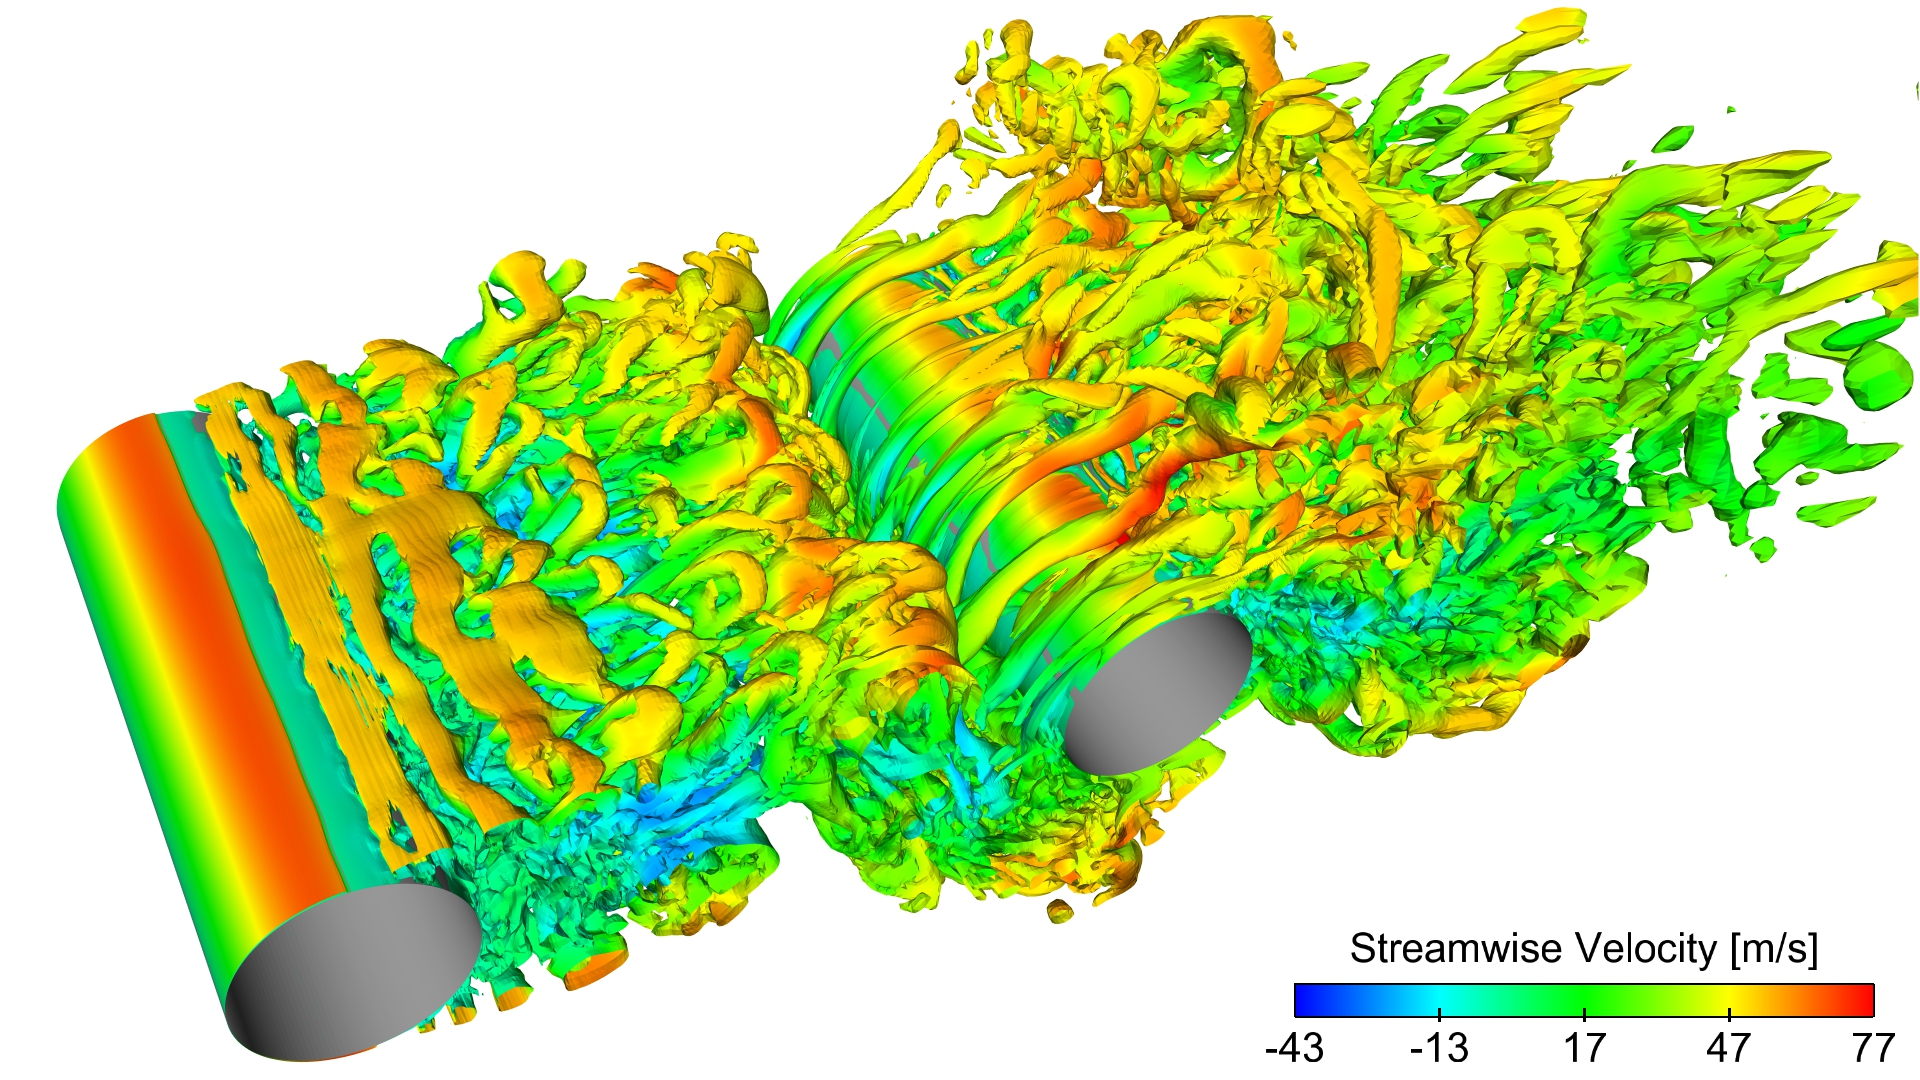
\includegraphics[width=0.40\textwidth]{tc_q_criteria}
    \bicaption{Q判据等值面图,同时测试一下一个很长的标题,比如这真的是一个很长很长很长很长很长很长很长很长的标题。}{Isocontour of Q criteria, at the same time, this is to test a long title, for instance, this is a really very long very long very long very long very long title.}
    \label{fig:tc_q_criteria}
\end{figure}

如果插图的空白区域过大,以图片\verb|shock_cyn|为例,自动裁剪如图\ref{fig:shock_cyn}。
\begin{figure}[!htbp]
    \centering
    %trim option's parameter order: left bottom right top
    % 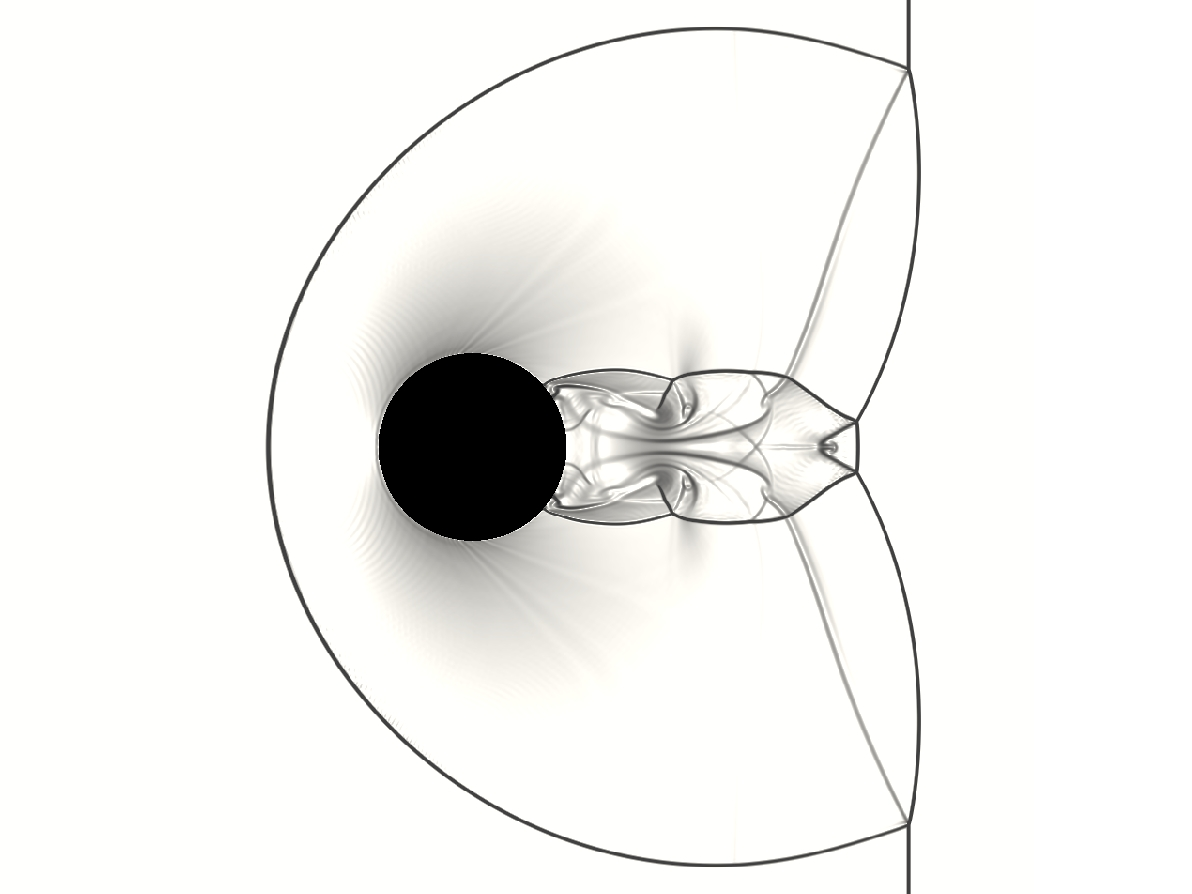
\includegraphics[trim = 30mm 0mm 30mm 0mm, clip, width=0.40\textwidth]{shock_cyn}
    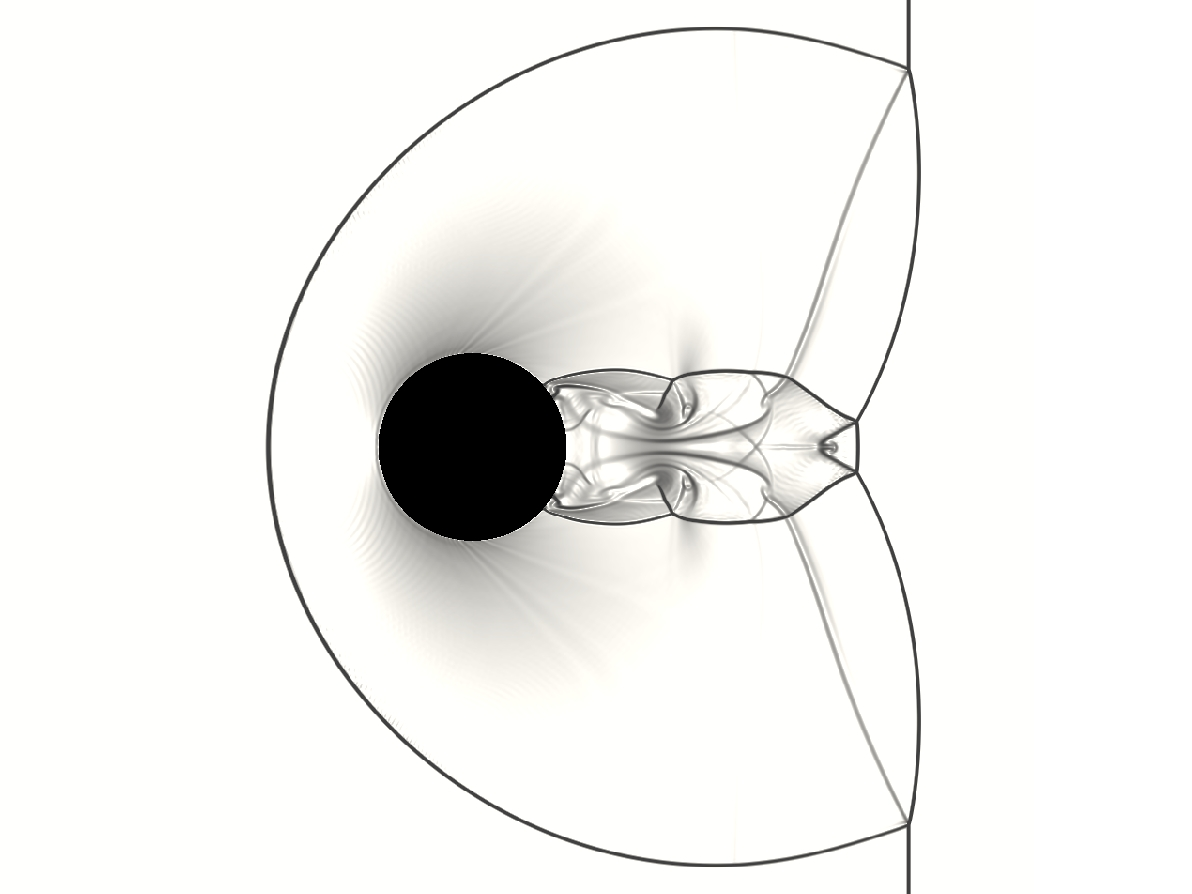
\includegraphics[width=0.40\textwidth]{shock_cyn}
    \bicaption{激波圆柱作用。}{Shock-cylinder interaction.}
    \label{fig:shock_cyn}
\end{figure}

多图的插入如图\ref{fig:oaspl},多图不应在子图中给文本子标题,只要给序号,并在主标题中进行引用说明。
\begin{figure}[!htbp]
    \centering
    \begin{subfigure}[b]{0.35\textwidth}
      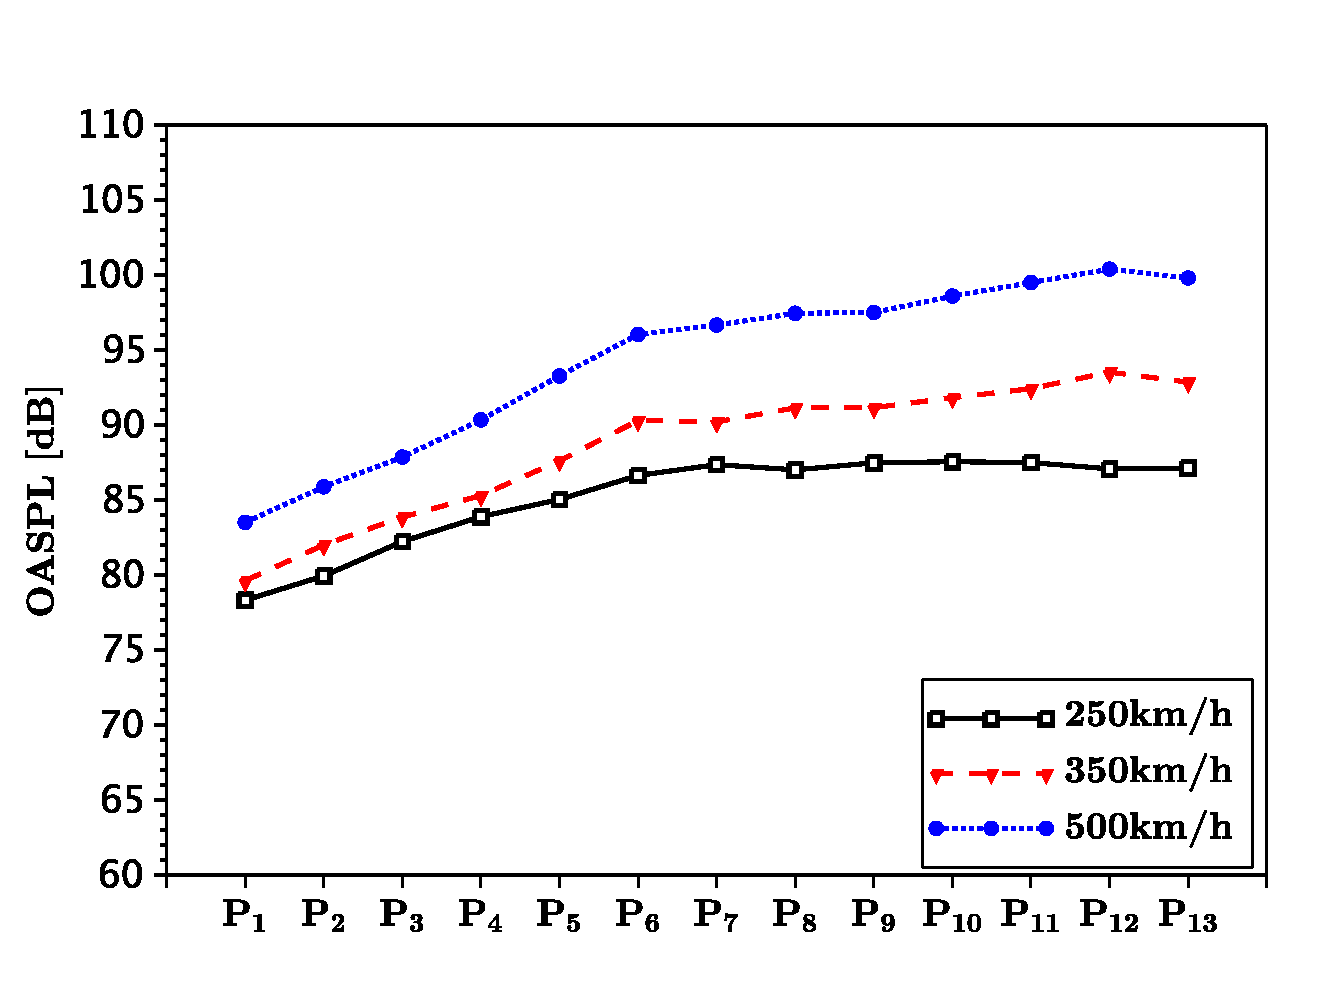
\includegraphics[width=\textwidth]{oaspl_a}
      \caption{}
      \label{fig:oaspl_a}
    \end{subfigure}%
    ~%add desired spacing
    \begin{subfigure}[b]{0.35\textwidth}
      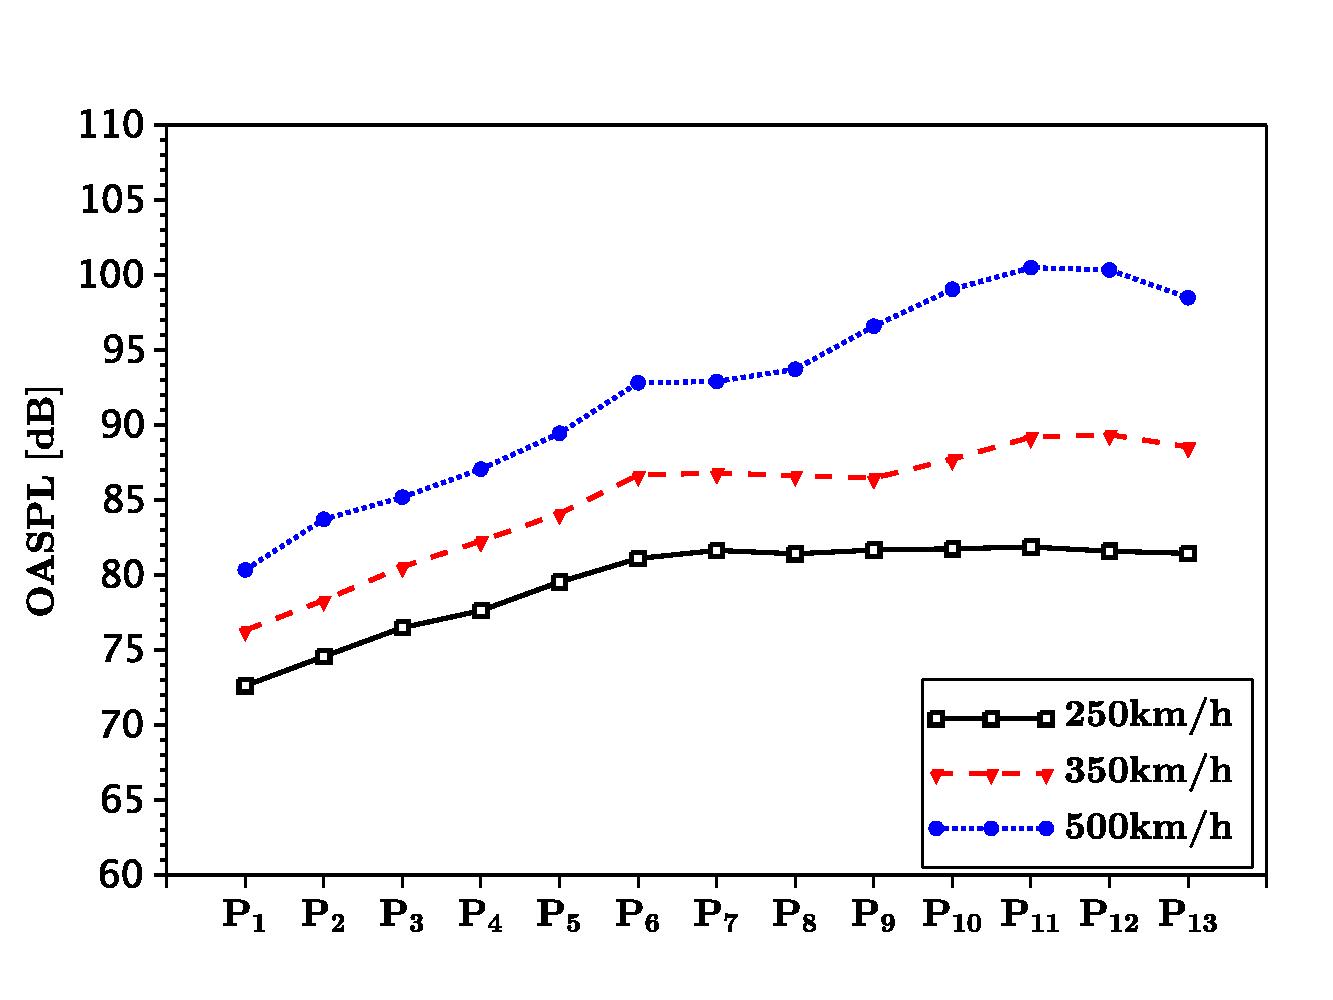
\includegraphics[width=\textwidth]{oaspl_b}
      \caption{}
      \label{fig:oaspl_b}
    \end{subfigure}
    \begin{subfigure}[b]{0.35\textwidth}
      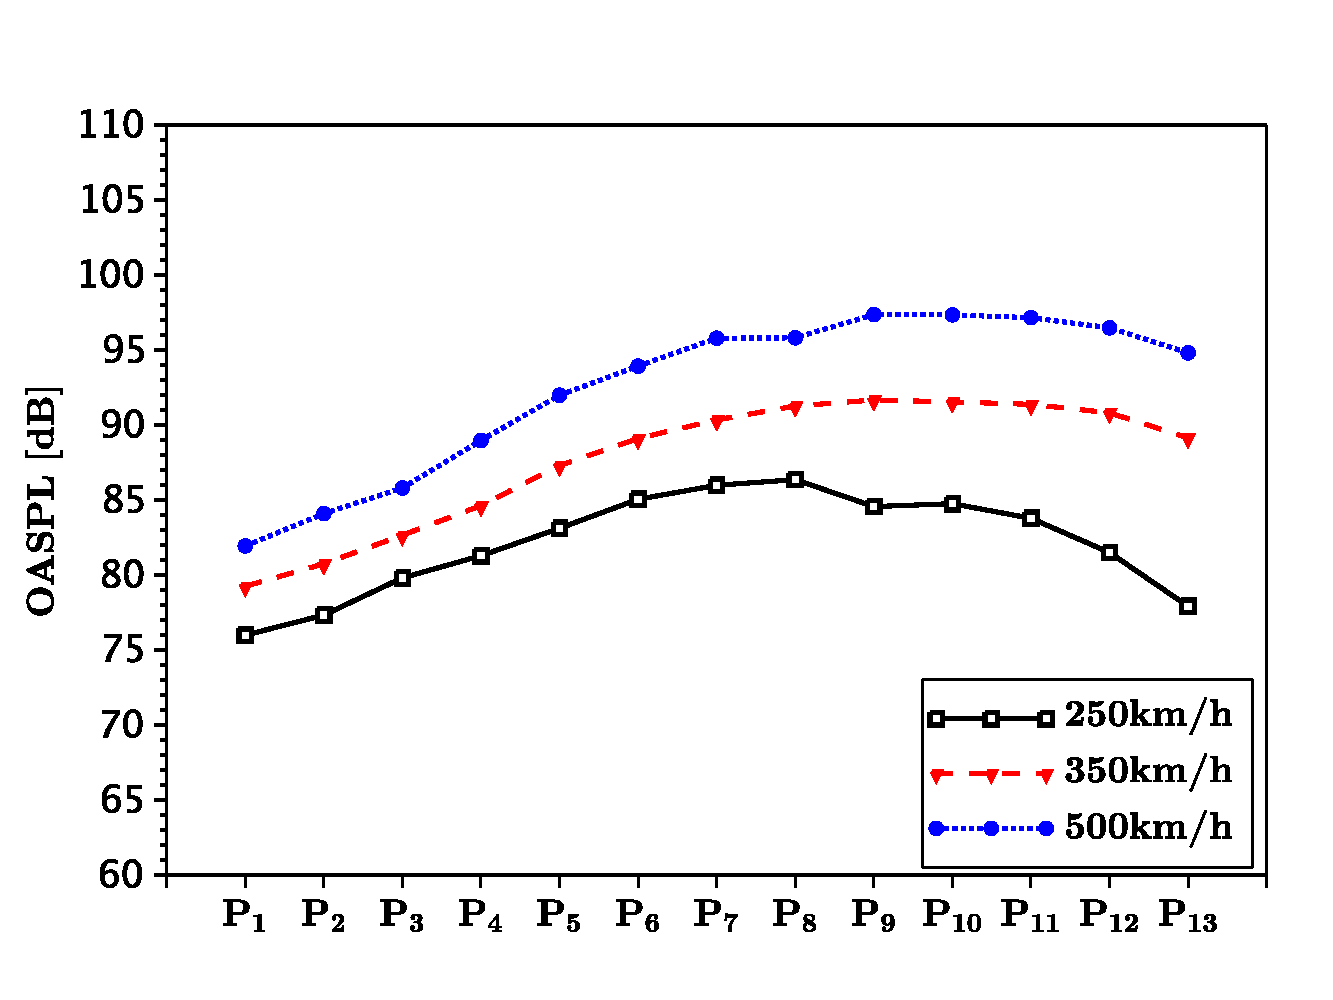
\includegraphics[width=\textwidth]{oaspl_c}
      \caption{}
      \label{fig:oaspl_c}
    \end{subfigure}%
    ~%add desired spacing
    \begin{subfigure}[b]{0.35\textwidth}
      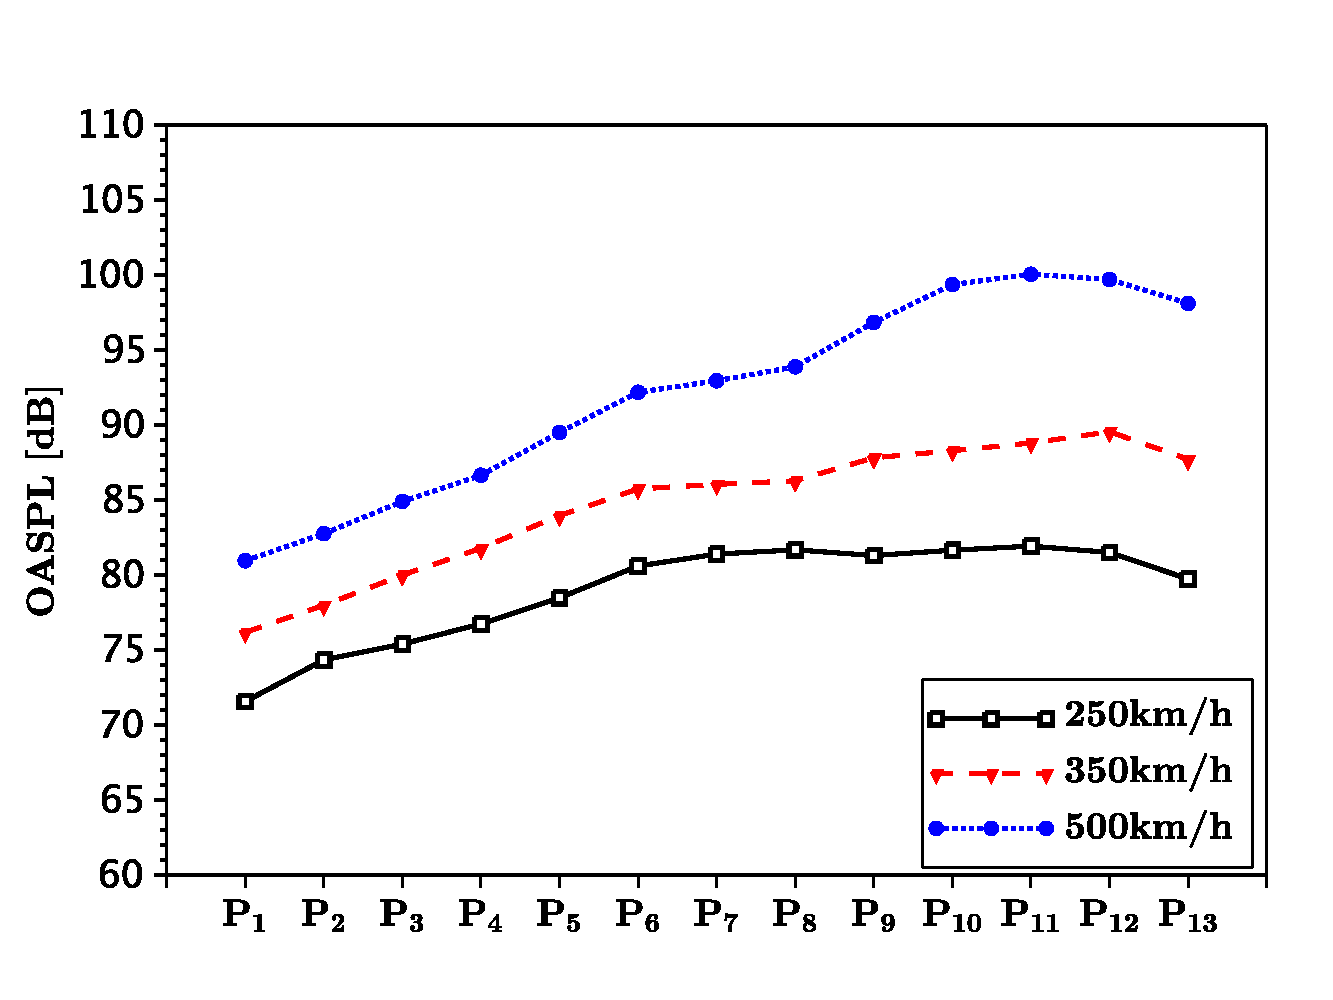
\includegraphics[width=\textwidth]{oaspl_d}
      \caption{}
      \label{fig:oaspl_d}
    \end{subfigure}
    \bicaption{总声压级。(a) 这是子图说明信息,(b) 这是子图说明信息,(c) 这是子图说明信息,(d) 这是子图说明信息。}{OASPL.(a) This is the explanation of subfig, (b) This is the explanation of subfig, (c) This is the explanation of subfig, (d) This is the explanation of subfig.}
    \label{fig:oaspl}
\end{figure}

\subsubsection{表}
表的一般格式是数据依序竖排,内容和项目由左至右横读,通版排版。表号也用章序号编码,如:表2.1是第2章中的第1表。表应有表题,与表号之间空1~2字,置于表的上方居中,用5号宋体,须全文统一。表中的内容和项目字号不大于图题的字号。

请见表~\ref{tab:sample}。制表的更多范例,请见 \href{https://en.wikibooks.org/wiki/LaTeX/Tables}{WiKibook Tables}。
\begin{table}[!htbp]
    \bicaption{这是一个样表。}{This is a sample table.}
    \label{tab:sample}
    \centering
    \footnotesize% fontsize
    \setlength{\tabcolsep}{4pt}% column separation
    \renewcommand{\arraystretch}{1.2}%row space 
    \begin{tabular}{lcccccccc}
        \hline
        Row number & \multicolumn{8}{c}{This is a multicolumn} \\
        %\cline{2-9}% partial hline from column i to column j
        \hline
        Row 1 & $1$ & $2$ & $4$ & $5$ & $6$ & $7$ & $8$\\
        Row 2 & $1$ & $2$ & $4$ & $5$ & $6$ & $7$ & $8$\\
        Row 3 & $1$ & $2$ & $4$ & $5$ & $6$ & $7$ & $8$\\
        Row 4 & $1$ & $2$ & $4$ & $5$ & $6$ & $7$ & $8$\\
        \hline
    \end{tabular}
\end{table}


\subsubsection{公式}
公式包括数学、物理和化学公式。正文中引用的公式、算式或方程式等可以按章序号用阿拉伯数字编号(式号),如:式(2.1)表示第2章第1式,公式一般单行居中排版与上下文分开,式号与公式同行居右排版。

比如勾股定理:
\begin{equation}
    a^2+b^2=c^2
\end{equation}

数学公式常用命令请见 \href{https://en.wikibooks.org/wiki/LaTeX/Mathematics}{WiKibook Mathematics}。artracom.sty中对一些常用数据类型如矢量矩阵等进行了封装,这样的好处是如有一天需要修改矢量的显示形式,只需单独修改artracom.sty中的矢量定义即可实现全文档的修改。

\subsubsection{算法}

如见算法~\ref{alg:euclid},详细使用方法请参见文档 \href{https://ctan.org/pkg/algorithmicx?lang=en}{algorithmicx}。

\begin{algorithm}[!htbp]
    \small
    \caption{Euclid's algorithm}\label{alg:euclid}
    \begin{algorithmic}[1]
        \Procedure{Euclid}{$a,b$}\Comment{The g.c.d. of a and b}
        \State $r\gets a\bmod b$
        \While{$r\not=0$}\Comment{We have the answer if r is 0}
        \State $a\gets b$
        \State $b\gets r$
        \State $r\gets a\bmod b$
        \EndWhile\label{euclidendwhile}
        \State \textbf{return} $b$\Comment{The gcd is b}
        \EndProcedure
    \end{algorithmic}
\end{algorithm}

\subsection{附录}
附录中的图、表、公式、参考文献等另行编排序号,与正文分开,也一律用阿拉伯数字编号,但在数码前冠以附录序码。例如:图A.1,式(B.3)等。
\subsection{计量单位}
学位论文一律采用1984年2月27日国务院发布的《中华人民共和国法定计量单位》,并遵照《中华人民共和国法定计量单位使用方法》执行。论文中命名用各种量、单位和符号,必须遵循国家标准GB3100-82,GB3101-82,GB3102/1-13-82等的规定。

单位名称和符号的书写方式,可以采用国际通用符号,也可以用中文名称,但统一采用一种,不要混用。

\subsection{参考文献}

参考文献引用过程以实例进行介绍,假设需要引用名为"Document Preparation System"的文献,步骤如下:

1)使用Google Scholar搜索Document Preparation System,在目标条目下点击Cite,展开后选择Import into BibTeX打开此文章的BibTeX索引信息,将它们copy添加到ref.bib文件中(此文件位于Biblio文件夹下)。

2)索引第一行 \verb|@article{lamport1986document,|中 \verb|lamport1986document| 即为此文献的label (\textbf{中文文献也必须使用英文label},一般遵照:姓氏拼音+年份+标题第一字拼音的格式),想要在论文中索引此文献,有两种索引类型:

文本类型:\verb|\citet{lamport1986document}|。正如此处所示 \citet{lamport1986document}; 

括号类型:\verb|\citep{lamport1986document}|。正如此处所示 \citep{lamport1986document}。

\textbf{多文献索引用英文逗号隔开}:

\verb|\citep{lamport1986document, chu2004tushu, chen2005zhulu}|。正如此处所示 \citep{lamport1986document,chu2004tushu,chen2005zhulu}

更多例子如:

\citet{walls2013drought}根据...的研究,首次提出...。其中关于...\citep{walls2013drought},是当前中国...得到迅速发展的研究领域\citep{chen1980zhongguo}。引用同一著者在同一年份出版的多篇文献时,在出版年份之后用
英文小写字母区别,如:\citep{yuan2012lana,yuan2012lanb,yuan2012lanc}。同一处引用多篇文献时,按出版年份由近及远依次标注,中间用
分号分开。例如\citep{chen1980zhongguo,stamerjohanns2009mathml,hls2012jinji,niu2013zonghe}。

使用著者-出版年制(authoryear)式参考文献样式时,中文文献必须在BibTeX索引信息的 \textbf{key} 域(请参考ref.bib文件)填写作者姓名的拼音,才能使得文献列表按照拼音排序。参考文献表中的条目(不排序号),先按语种分类排列,语种顺 序是:中文、日文、英文、俄文、其他文种。然后,中文按汉语拼音字母顺序排列,日文按第一著者的姓氏笔画排序,西文和 俄文按第一著者姓氏首字母顺序排列。如中\cite{niu2013zonghe}、日\cite{Bohan1928}、英\cite{stamerjohanns2009mathml}、俄\cite{Dubrovin1906}。

如此,即完成了文献的索引,请查看下本文档的参考文献一章,看看是不是就是这么简单呢?是的,就是这么简单!

不同文献样式和引用样式,如著者-出版年制(authoryear)、顺序编码制(numbers)、上标顺序编码制(super)可在Thesis.tex中对artratex.sty调用实现,如:
\begin{itemize}
    \footnotesize
    \item \verb+\usepackage[numbers]{artratex}+ $\%$ 文本: Jones [1]; 括号: [1]
    \item \verb+\usepackage[super]{artratex}+ $\%$ 文本: Jones 上标[1]; 括号: 上标[1]
    \item \verb+\usepackage[authoryear]{artratex}+ $\%$ 文本: Jones (1995); 括号: (Jones, 1995)
    \item \verb+\usepackage[alpha]{artratex}+ $\%$ 文本: 不可用; 括号: [Jon95]
\end{itemize}

当前文档的默认参考文献样式为\textbf{authoryear}。若在上标(\textbf{super})模式下,希望在特定位置将上标改为嵌入式标,可使用

文本类型:\verb|\citens{lamport1986document,chen2005zhulu}|。

正如此处所示\cite{lamport1986document,chen2005zhulu}

括号类型:\verb|\citens{lamport1986document,chen2005zhulu}|。

正如此处所示\cite{lamport1986document,chen2005zhulu}

参考文献索引更为详细的信息,请见 \href{https://github.com/zepinglee/gbt7714-bibtex-style}{zepinglee} 和 \href{https://en.wikibooks.org/wiki/LaTeX/Bibliography_Management}{WiKibook Bibliography}。


参考文献采用顺序号编号体系。

专著格式: 

[序号] 编著者. 书名[M]. 出版地:出版社,年代,起止页码.

期刊论文格式: 

[序号] 作者. 论文名称[J]. 期刊名称,年度,卷(期):起止页码.

学位论文格式: 

[序号] 作者. 学位论文名称[D]. 发表地:学位授予单位,年度.

参考文献举例: 

[1] 张毅. 铸造工艺CAD及其应用[M]. 北京:机械工业出版社,1994,14-15. 

[2] Huang S C, Huang Y M, Shieh S M. Vibration and stability of a rotating shaft containing a transerse crack [J]. J Sound and Vibration, 1993, 162(3): 387-401.

[3] 周丽. 机械式挖掘机工作装置的优化与仿真[D]. 沈阳:东北大学,2000.


\subsection{攻读博士学位期间取得的学术成果}

期刊格式:
[序号] 作者. 论文名称[J]. 期刊名称,年度,卷(期):起止页码. (检索情况)(对应论文章
节)

专利格式:

[序号] 专利申请者. 专利题名:专利国别,专利号[P]. 发布日期. (对应论文章节)

示例:

[1] Huang S C, Huang Y M, Shieh S M. Vibration and stability of a rotating shaft containing a transerse crack[J]. J Sound and Vibration, 1993, 162(3): 387-401. (SCI检索)(对应论文第四章)

[2] 高航,张立成,周士昌. 高压辊磨机液压系统及其动态特性[J]. 东北大学学报,2000,21(1):38-40. (EI检索)(对应论文第五章)

[3] 刘加林. 多功能一次性压舌板:中国,92214985.2[P]. 1993-04-14. (对应论文第四章)


注:双盲评审版学位论文中须隐去所有作者(申请者)姓名,仅标注排序即可。

示例:

[1] 第一作者. Vibration and stability of a rotating shaft containing a transerse crack[J]. J Sound and Vibration, 1993, 162(3): 387-401. (SCI检索)(对应论文第四章)

[2] 第二作者. 高压辊磨机液压系统及其动态特性[J]. 东北大学学报,2000,21(1):38-40. (EI检索)(对应论文第五章)

[3] 第二排序. 多功能一次性压舌板:中国,92214985.2[P]. 1993-04-14. (对应论文第四章)





% \chapter{LaTeX使用说明}\label{chap:guide}

为方便使用及更好地展示LaTeX排版的优秀特性,neuthesis的框架和文件体系进行了细致地处理,尽可能地对各个功能和板块进行了模块化和封装,对于初学者来说,众多的文件目录也许一开始让人觉得有些无所适从,但阅读完下面的使用说明后,会发现原来使用思路是简单而清晰的,而且,当对LaTeX有一定的认识和了解后,会发现其相对Word类排版系统极具吸引力的优秀特性。所以,如果是初学者,请不要退缩,请稍加尝试和坚持,以领略到LaTeX的非凡魅力,并可以通过阅读相关资料如LaTeX Wikibook\cite{wikibook2014latex}来完善自己的使用知识。

\section{先试试效果}

\begin{enumerate}
    \item 安装软件:根据所用操作系统和章节~`\ref{sec:system}`中的信息安装LaTeX编译环境。
    \item 获取模板:下载 \href{https://github.com/mervin0502/neuthesis}{neuthesis} 模板并解压。neuthesis模板不仅提供了相应的类文件,同时也提供了包括参考文献等在内的完成学位论文的一切要素,所以,下载时,推荐下载整个neuthesis文件夹,而不是单独的文档类。
    \item 编译模板:
        \begin{enumerate}
            \item Windows:双击运行artratex.bat脚本。
            \item Linux或MacOS: {\scriptsize \verb|terminal| -> \verb|chmod +x ./artratex.sh| -> \verb|./artratex.sh xa|}
            \item 任意系统:都可使用LaTeX编辑器打开Thesis.tex文件并选择xelatex编译引擎进行编译。
        \end{enumerate}
    \item 错误处理:若编译中遇到了问题,请先查看“常见问题”(章节~\ref{sec:qa})。
\end{enumerate}

编译完成即可获得本PDF说明文档。而这也完成了学习使用neuthesis撰写论文的一半进程。什么?这就学成一半了,这么简单???,是的,就这么简单!

\section{文档目录简介}

\subsection{Thesis.tex}

Thesis.tex为主文档,其设计和规划了论文的整体框架,通过对其的阅读可以了解整个论文框架的搭建。

\subsection{编译脚本}

\begin{itemize}
    \item Windows:双击Dos脚本artratex.bat可得全编译后的PDF文档,其存在是为了帮助不了解LaTeX编译过程的初学者跨过编译这第一道坎,请勿通过邮件传播和接收此脚本,以防范Dos脚本的潜在风险。
    \item Linux或MacOS:在terminal中运行
        \begin{itemize}
            \item \verb|./artratex.sh xa|:获得全编译后的PDF文档
            \item \verb|./artratex.sh x|:快速编译模式
        \end{itemize}
    \item 全编译指运行 \verb|xelatex+bibtex+xelatex+xelatex| 以正确生成所有的引用链接,如目录,参考文献及引用等。在写作过程中若无添加新的引用,则可用快速编译,即只运行一遍LaTeX编译引擎以减少编译时间。
\end{itemize}

\subsection{Tmp文件夹}

运行编译脚本后,编译所生成的文档皆存于Tmp文件夹内,包括编译得到的PDF文档,其存在是为了保持工作空间的整洁,因为好的心情是很重要的。

\subsection{Style文件夹}

包含neuthesis文档类的定义文件和配置文件,通过对它们的修改可以实现特定的模版设定。若需更新模板,一般只需用新的样式文件替换旧的即可。

\begin{enumerate}
    \item neuthesis.cls:文档类定义文件,论文的最核心的格式即通过它来定义的。
    \item neuthesis.cfg:文档类配置文件,设定如目录显示为“目~录”而非“目录”。
    \item artratex.sty: 常用宏包及文档设定,如参考文献样式、文献引用样式、页眉页脚设定等。这些功能具有开关选项,常只需在Thesis.tex中的如下命令中进行启用即可,一般无需修改artratex.sty本身。
        
        \path{\usepackage[options]{artratex}} 
    \item artracom.sty:自定义命令以及添加宏包的推荐放置位置。
\end{enumerate}

\subsection{Tex文件夹}

文件夹内为论文的所有实体内容,正常情况下,这也是\textbf{使用neuthesis撰写学文论文时,主要关注和修改的一个位置,注:所有文件都必须采用UTF-8编码,否则编译后将出现乱码文本},详细分类介绍如下:

\begin{itemize}
    \item Frontpage.tex:为论文中英文封面及中英文摘要。\textbf{论文封面会根据英文学位名称如Bachelor,Master,或是Doctor自动切换为相应的格式}。
    \item Mainmatter.tex:索引需要出现的Chapter。开始写论文时,可以只索引当前章节,以快速编译查看,当论文完成后,再对所有章节进行索引即可。
    \item Chap{\_}xxx.tex:为论文主体的各个章节,可根据需要添加和撰写。
    \item Appendix.tex:为附录内容
    \item Backmatter.tex:为发表文章信息和致谢部分等。
\end{itemize}

\subsection{Img文件夹}

用于放置论文中所需要的图类文件,支持格式有:.jpg, .png, .pdf。其中,\verb|neu_logo.pdf|为东北大学校徽。不建议为各章节图片建子目录,即使图片众多,若命名规则合理,图片查询亦是十分方便。

\subsection{Biblio文件夹}

\begin{enumerate}
    \item ref.bib:参考文献信息库。
    \item gbt7714-xxx.bst:符合国标的文献样式定义文件。由 \href{https://github.com/zepinglee/gbt7714-bibtex-style}{zepinglee}  开发,并满足最新国标要求。与文献样式有关的问题,请查阅开发者所提供的文档,并建议适当追踪其更新。
\end{enumerate}

\section{常见使用问题}\label{sec:qa}

\begin{enumerate}
    \item 模板每次发布前,都已在Windows,Linux,MacOS系统上测试通过。下载模板后,若编译出现错误,则请见 \href{https://github.com/mervin0502/neuthesis/wiki}{neuthesis和LaTeX知识小站} 的 \href{https://github.com/mervin0502/neuthesis/wiki/%E7%BC%96%E8%AF%91%E6%8C%87%E5%8D%97}{编译指南}。

    \item 模板文档的编码为UTF-8编码。所有文件都必须采用UTF-8编码,否则编译后生成的文档将出现乱码文本。若出现文本编辑器无法打开文档或打开文档乱码的问题,请检查编辑器对UTF-8编码的支持。如果使用WinEdt作为文本编辑器(\textbf{不推荐使用}),应在其Options -> Preferences -> wrapping选项卡下将两种Wrapping Modes中的内容:
        
        TeX;HTML;ANSI;ASCII|DTX...
        
        修改为:TeX;\textbf{UTF-8|ACP;}HTML;ANSI;ASCII|DTX...
        
        同时,取消Options -> Preferences -> Unicode中的Enable ANSI Format。

    \item 推荐选择xelatex或lualatex编译引擎编译中文文档。编译脚本的默认设定为xelatex编译引擎。你也可以选择不使用脚本编译,如直接使用 LaTeX文本编辑器编译。注:LaTeX文本编辑器编译的默认设定为pdflatex编译引擎,若选择xelatex或lualatex编译引擎,请进入下拉菜单选择。为正确生成引用链接,需要进行全编译。

    \item Texmaker使用简介
        \begin{enumerate}
            \footnotesize
            \item 使用 Texmaker “打开 (Open)” Thesis.tex。
            \item 菜单 “选项 (Options)” -> “设置当前文档为主文档 (Define as Master Document)”
            \item 菜单 “自定义 (User)” -> “自定义命令 (User Commands)” -> “编辑自定义命令 (Edit User Commands)” -> 左侧选择 “command 1”,右侧 “菜单项 (Menu Item)” 填入 Auto Build -> 点击下方“向导 (Wizard)” -> “添加 (Add)”: xelatex + bibtex + xelatex + xelatex + pdf viewer -> 点击“完成 (OK)”
            \item 使用 Auto Build 编译带有未生成引用链接的源文件,可以仅使用 xelatex 编译带有已经正确生成引用链接的源文件。
            \item 编译完成,“查看(View)” PDF,在PDF中 “ctrl+click” 可链接到相对应的源文件。
        \end{enumerate}
    
    \item 模版的设计可能地考虑了适应性。致谢等所有条目都是通过最为通用的

        \verb+\chapter{item name}+  and \verb+\section*{item name}+

        来显式实现的 (请观察Backmatter.tex),从而可以随意添加,放置,和修改,如同一般章节。对于图表目录名称则可在neuthesis.cfg中进行修改。

    \item 设置文档样式: 在artratex.sty中搜索关键字定位相应命令,然后修改
        \begin{enumerate}
            \item 正文行距:启用和设置 \verb|\linespread{1.5}|,默认1.5倍行距。
            \item 参考文献行距:修改 \verb|\setlength{\bibsep}{0.0ex}|
            \item 目录显示级数:修改 \verb|\setcounter{tocdepth}{2}|
            \item 文档超链接的颜色及其显示:修改 \verb|\hypersetup|
        \end{enumerate}

    \item 文档内字体切换方法:
        \begin{itemize}
            \item 宋体:东北大学论文模板neuthesis 或 \textrm{东北大学论文模板neuthesis}
            \item 粗宋体:{\bfseries 东北大学论文模板neuthesis} 或 \textbf{东北大学论文模板neuthesis}
            \item 黑体:{\sffamily 东北大学论文模板neuthesis} 或 \textsf{东北大学论文模板neuthesis}
            \item 粗黑体:{\bfseries\sffamily 东北大学论文模板neuthesis} 或 \textsf{\bfseries 东北大学论文模板neuthesis}
            \item 仿宋:{\ttfamily 东北大学论文模板neuthesis} 或 \texttt{东北大学论文模板neuthesis}
            \item 粗仿宋:{\bfseries\ttfamily 东北大学论文模板neuthesis} 或 \texttt{\bfseries 东北大学论文模板neuthesis}
            \item 楷体:{\itshape 东北大学论文模板neuthesis} 或 \textit{东北大学论文模板neuthesis}
            \item 粗楷体:{\bfseries\itshape 东北大学论文模板neuthesis} 或 \textit{\bfseries 东北大学论文模板neuthesis}
        \end{itemize}

    \item 封面下划线上的文本不居中下划线,这是因为下划线前面还有字头,导致文本只能在页面居中和在下划线上居中二选一。当前封面采取页面居中。如需要调整文本在下划线上的位置,可用 \verb|\hspace{+/- n.0em}| 命令来插入或删除 n 个空格,进行手动调整,比如

        \verb|\advisor{\hspace{+3.0em} xxx~研究员~xxx单位}|
                
    有时下划线看上去粗细不一致,这是显示的问题,打印正常。
\end{enumerate}



%---------------------------------------------------------------------------%
% main content

% \layout
%-P

%-
%-> Backmatter: bibliography, glossary, index
%-
\backmatter% initialize the environment
\intotoc{\bibname}% add link to contents table and bookmark
% \bibliography{Biblio/ref}% bibliography
\makereference

\chapter[致谢]{致\quad 谢}\chaptermark{致\quad 谢}% syntax: \chapter[目录]{标题}\chaptermark{页眉}
% \thispagestyle{noheaderstyle}% 如果需要移除当前页的页眉
%\pagestyle{noheaderstyle}% 如果需要移除整章的页眉

\reviewORprint{
}{
    (致谢)
}

\chapter{攻读博士学位期间取得的学术成果}

\section*{个人简历:}


\reviewORprint{
    \section*{第一作者发表/录用学术论文:}
    \begin{enumerate}[leftmargin=*]
        \item Title[J]Journal, Year, Volume(Number):Pages. (\textbf{SCI, JCR1, 论文第三章})
    \end{enumerate}
    \section*{第一作者在审学术论文:}
    \begin{enumerate}[leftmargin=*]
        \item Title[J]Journal, Year, Volume(Number):Pages. (\textbf{SCI, JCR1, 论文第三章})
    \end{enumerate}
    \section*{通讯作者发表/录用学术论文:}
    \begin{enumerate}[leftmargin=*]
        \item Title[J]Journal, Year, Volume(Number):Pages. (\textbf{SCI, JCR1, 第二作者/通讯作者})
    \end{enumerate}
    \section*{合作作者发表/录用学术论文:}
    \begin{enumerate}[leftmargin=*]
        \item Title[J]Journal, Year, Volume(Number):Pages. (\textbf{SCI, JCR1, 第二作者})
    \end{enumerate}
}{
    \section*{学术论文:}
    \begin{enumerate}[leftmargin=*]
        \item Authors. Title[J]Journal, Year, Volume(Number):Pages.
    \end{enumerate}
}

\section*{科研项目:}

\begin{enumerate}[leftmargin=*]
    \item 项目类型,项目号, 项目名称, 日期。
\end{enumerate}

\cleardoublepage[plain]% 让文档总是结束于偶数页,可根据需要设定页眉页脚样式,如 [noheaderstyle]

% other information
% \showthe\artxfontset
\end{document}
%---------------------------------------------------------------------------%

